\section{MIP model}
For the MIP model we choose themsolver-independent language AMPL. Taking inspiration from the AMPL book, we developed our model around the idea to use a binary tensor that encodes the travel of each courier through all the possible delivery point, starting and ending at the depot. This travel is an Hamiltonian cycle and we recall here the definition:
\begin{definition}[Hamiltonian cycle]
In the mathematical field of graph theory an Hamiltonian cycle (or Hamiltonian circuit) is a cycle that visits each vertex exactly once.
\end{definition}
In order to preserve the properties of the Hamiltonian cycle and to avoid the possible presence of sub-circuits we added some constraints, and in particular for the last case we followed the Miller–Tucker–Zemlin (MTZ) approach.\\
The work-flow was based on the construction of three different models: the initial-one, the implied-one, with the adding of the implied constraint, and the symmetry-one, with the adding of the symmetry breaking constraint. The purpose is to show how the adding of this two constraints could improve the performance in terms of execution time and number of simplex-iterations or branching nodes explored.

\subsection{Decision variables}
The models are based on the following three variables:
\begin{itemize}
    \item A binary tensor $X \in \{0,1\}^{(n+1) \times (n+1) \times m}$, where $X[i,j,k] = 1$ if and only if the courier $k$ depart from the $i-th$ delivery point and arrive at the $j-th$ one. The column and row $n+1$ stand for the depot. 
    \item A binary matrix $A \in \{0,1\}^{n \times m}$, where $A[i,k] = 1$ if and only if the the package $i$ is delivered by the courier $k$.\\
    We observe that this kind of variable is not strictly necessary for the model, but it allowed us to write some constraints in an easier way.
    \item An auxiliary matrix $u \in \{1,\dots,n+1\}^{(n+1) \times m}$ that keeps track of the order in which nodes are visited by each courier starting from the point $1$. It is necessary, following the MTZ formulation, for the sub-circuits elimination. The interpretation is that, fixing the courier $k$, $u[i,k] < u[j,k]$ implies that the node $i$ is visited before the node $j$ by the courier $k$.
\end{itemize}


\subsection{Objective function}
As objective function, defined from the assignment as the maximum distance travelled by any courier, we used $\max_{k \in 1 \dots m}\sum_{i = 1}^{n+1} X[i,j,k]D[i,j]$ with the goal to minimize it. As upper bound we chose the sum over all the indexes of the matrix $D$: $\sum_{i,j = 1}^{n+1} D[i,j]$. Instead as lower bound we chose the maximum distance travelled picking only one package: $\max_{i \in 1 \dots n} (D[n+1,i] + D[i,n+1])$. In fact, due to the triangular inequality, if another package is picked up by the courier the distance will grow. 

\subsection{Constraints}
\begin{itemize}
    \item We defined the constraints that link the variables $A$ and $X$:
    \begin{equation}
        \sum_{j = 1}^{n+1} X[i,j,k] = A[i,k]  \qquad  \forall i \in 1 \dots n,\forall k \in 1 \dots m.
    \end{equation}
    \begin{equation}
        \sum_{i = 1}^{n+1} X[i,j,k] = A[j,k]  \qquad  \forall j \in 1 \dots n,\forall k \in 1 \dots m.
    \end{equation}

    \item We defined the constraint that specify that each package has to be assigned:
    \begin{equation}
        \sum_{k = 1}^{m} A[i,k] = 1  \qquad \forall i \in 1 \dots n.
    \end{equation}

    \item We defined the constraint concerned the capacity of each courier:
    \begin{equation}
        \sum_{i = 1}^{n} A[i,k] s[i] \leq l[k] \qquad \forall k \in 1 \dots m.
    \end{equation}

    \item We defined the constraint that avoid that each courier depart and and arrive at the same point.
    \begin{equation}
        X[i,i,k] = 0 \qquad \forall i \in 1 \dots n+1, \forall k \in 1 \dots m.
    \end{equation}

    \item We defined two constraints that ensure respectively that there is one arrival and one departure for each node. This concerns only to the internal nodes, because the depot is visited by each courier. 
    \begin{equation}
        \sum_{i \in 1 \dots n+1, k \in 1 \dots m} X[i,j,k] = 1 \qquad \forall j \in 1 \dots n.  
    \end{equation}
    \begin{equation}
        \sum_{j \in 1 \dots n+1, k \in 1 \dots m} X[i,j,k] = 1 \qquad \forall i \in 1 \dots n.  
    \end{equation}

    \item We defined one constraint that allows the preservation of the flow (if one courier arrives at one node, he departs from the same one):
    \begin{equation}
        \sum_{i = 1}^{n+1} X[i,j,k] = \sum_{i = 1}^{n+1} X[j,i,k] \qquad \forall j \in 1 \dots n, \forall k \in 1 \dots m.
    \end{equation}

    \item We defined two constraints that ensures that each courier starts and end his travel at the depot:
    \begin{equation}
        \sum_{j = 1}^{n} X[n+1,j,k] = 1 \qquad \forall k \in 1 \dots m.
    \end{equation}
    \begin{equation}
        \sum_{j = 1}^{n} X[j,n+1,k] = 1 \qquad \forall k \in 1 \dots m.
    \end{equation}

    \item Following the MTZ formulation we wrote three constraints in order to avoid sub-circuits:
    \begin{equation}
        u[i,k] - u[j,k] + 1 \leq n(1 - X[i,j,k]) \qquad \forall i \in 1 \dots n, \forall j \in 1 \dots n+1, \forall k \in 1 \dots m.
    \end{equation}
    \begin{equation}
        u[i,k] \leq X[n+1,i,k] + (n+1)(1-X[n+1,i,k]) \qquad \forall i \in 1 \dots n, \forall k \in 1 \dots m.
    \end{equation}
    \begin{equation}
        u[j,k] \geq (u[i,k] + 1)X[i,j,k] \qquad \forall i \in 1 \dots n, \forall j \in 1 \dots n+1, \forall k \in 1 \dots m.
    \end{equation}

    \subsubsection{Implied Model}
    For the implied model we added one more constraint:
    \begin{equation}
        \sum_{i = 1}^{n} A[i,k] \geq 1 \qquad \forall k \in 1 \dots m.
    \end{equation}
    The meaning of this implied constraint is that every couriers has to bring at least one package. This information is not explicitly wrote in the assignment but it could significantly help to reach the optimal solution, being one necessary condition. Our claim is the following:
    \begin{lem}
    If the solution is optimal then every courier has to bring at least one package.
    \end{lem}
    \begin{proof}
    Let's assume for the sake of contradiction that we have found an optimal solution where there are one or plus couriers which don't bring any package, calling him $k_1$. Let's suppose that the courier $k_j$ is the one that cover the maximum distance $D_j$. If we assign one package, calling $i$, that $k_j$ brought, to $k_1$ then, due to the triangular inequality, the two new distances, $D_1$, travelled by the courier $k_1$, and $D_2$, travelled by the courier $k_j$, are less or equal to $D_j$, in fact:
    \begin{equation}
    D_1 = D[depot,i] + D[i,depot] \leq D[depot, i_1] + \dots + D[i_r, i] + D[i, i_s] + \dots + D[i_t, depot] = D_j.
    \end{equation}
    \begin{align}
    D_2 = D[depot,i_1] + \dots D[i_r,i_s] + \dots D[i_t, depot] \leq D[depot, i_1]
    + \dots \\
    \dots + D[i_r, i] + D[i, i_s] + \dots + D[i_t, depot] = D_j.
    \end{align}
    Therefore, $D_j$ is not an optimal solution and we have found a contradiction.
    \end{proof}
    
    \subsubsection{Symmetry Model}
    For the symmetry model we added the symmetry-breaking constraint related to the number of packages brought by couriers with the same capacity:
    \begin{equation}
    \sum_{i = 1}^{n} A[i,k] \leq \sum_{i = 1}^n A[i,j],
    \end{equation}
    where $k,j \in 1, \dots, m$ with $k < j$ and $l[k] = l[j]$.
\end{itemize}


\subsection{Validation}

\subsubsection{Experimental design}
For reason of repeatability, we decided to use only open-access solver, HIGHS and SCIP, given by the AMPL framework.
Both SCIP and HIGHS give us the information related to the number of simplex iterations performed and branching nodes explored. From what we have understood this is due to the fact that they try to initially solve the relaxed-version of the problem (LP) using the revised simplex-method and finding a lower bound for the solution; then, if the solution found is not integer, they start to solve the MIP part using brunch and cut (SCIP) or brunch and bound (HIGHS). For the resolution of the sub-problems generated by these two methods, they proceed as before, starting from relaxation to successively pass to MIP.

\subsubsection{Experimental results}

For the first ten instances we plotted three graphs about the execution time (in seconds), the number of simplex iterations and branching nodes explored by the two solvers.
\begin{figure}[H]
    \centering
    \begin{subfigure}{0.3\linewidth}
        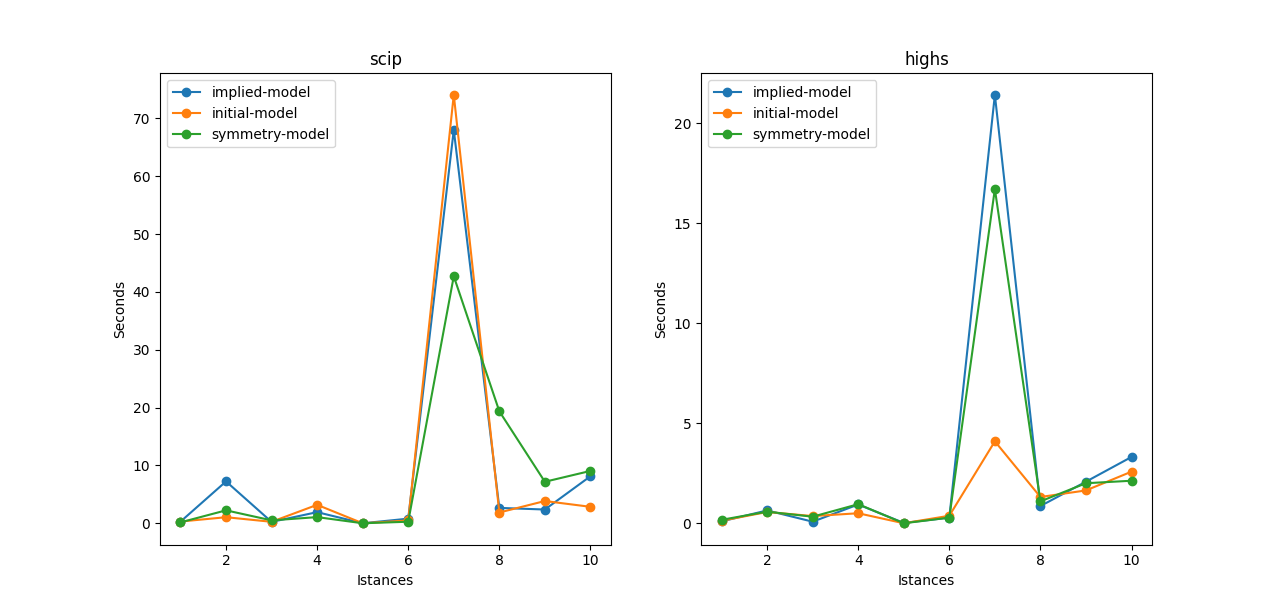
\includegraphics[width=\textwidth]{img/mip/execution_time_2.png}
    \end{subfigure}
    \begin{subfigure}{0.3\linewidth}
        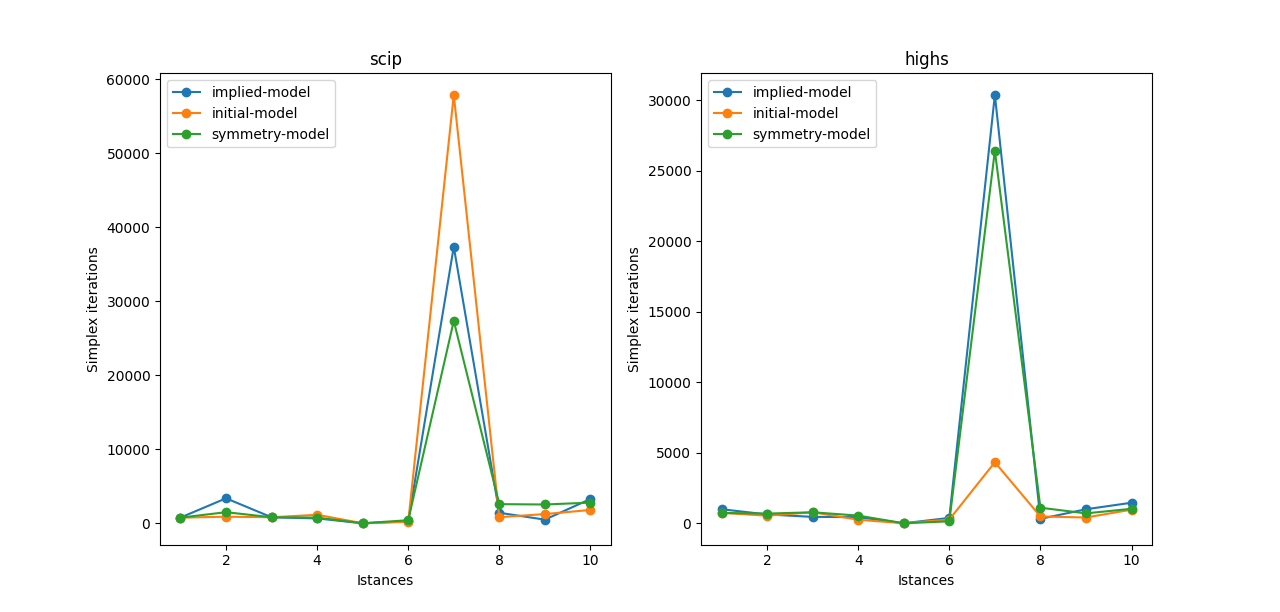
\includegraphics[width=\textwidth]{img/mip/simplex_iterations_2.png}
    \end{subfigure}
    \begin{subfigure}{0.3\linewidth}
        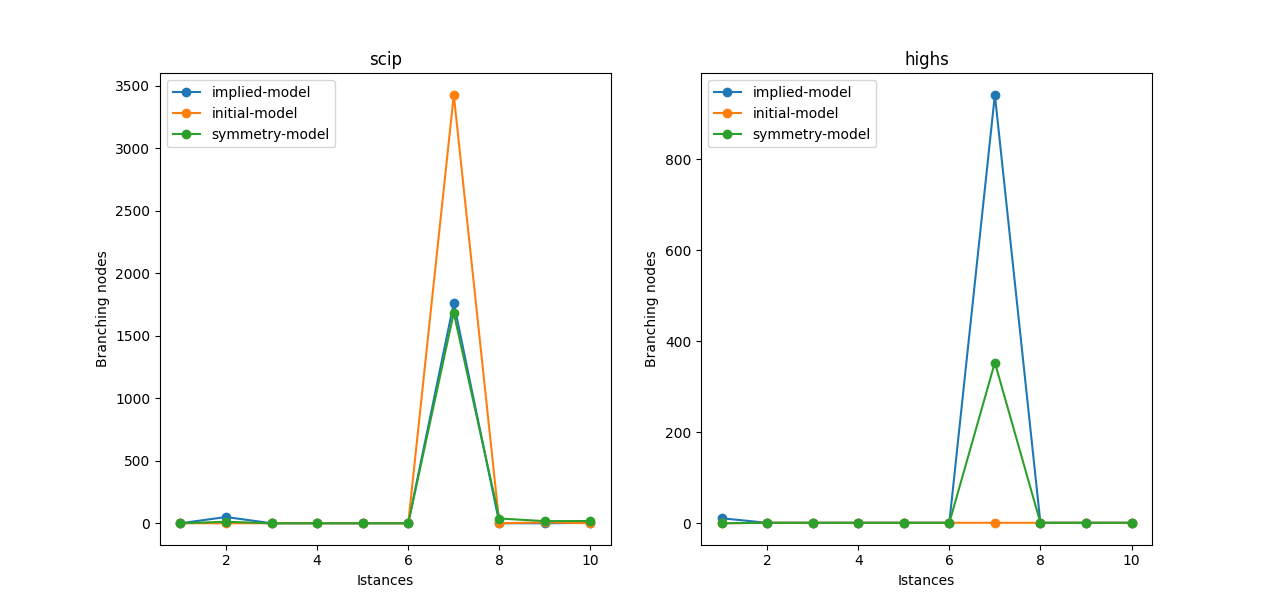
\includegraphics[width=\textwidth]{img/mip/Figure_2.png}
    \end{subfigure}
    \caption{Compared statistics of the performances of the three models, divided by SCIP and HIGHS solvers}
\end{figure}

We can observe that, while for the SCIP solver the adding of the implied and symmetry breaking constraint improve the performance, it's not the same for HIGHS.
But the HIGHS performances are in general significantly better than the SCIP ones.


Instead here we include the table with all the results given by the two solvers and the three models for all the instances.

\begin{table}[H]
        \centering
        \caption{Results of the scip and highs solvers for the three models}
        \resizebox{\textwidth}{!}{
        \begin{tabular}{ccccccc}
                \toprule
                Id & initial-model-scip & initial-model-highs & implied-model-scip & implied-model-highs & symmetry-model-scip & symmetry-model-highs \\ 
                \midrule
                1 & \textbf{14} &       \textbf{14} &   \textbf{14} &   \textbf{14} &   \textbf{14} &   \textbf{14} \\ 
                2 & \textbf{226} &      \textbf{226} &  \textbf{226} &  \textbf{226} &  \textbf{226} &  \textbf{226} \\

                3 & \textbf{12} &       \textbf{12} &   \textbf{12} &   \textbf{12} &   \textbf{12} &   \textbf{12} \\ 
                4 & \textbf{220} &      \textbf{220} &  \textbf{220} &  \textbf{220} &  \textbf{220} &  \textbf{220} \\

                5 & \textbf{206} &      \textbf{206} &  \textbf{206} &  \textbf{206} &  \textbf{206} &  \textbf{206} \\

                6 & \textbf{322} &      \textbf{322} &  \textbf{322} &  \textbf{322} &  \textbf{322} &  \textbf{322} \\

                7 & \textbf{167} &      \textbf{167} &  \textbf{167} &  \textbf{167} &  \textbf{167} &  \textbf{167} \\

                8 & \textbf{186} &      \textbf{186} &  \textbf{186} &  \textbf{186} &  \textbf{186} &  \textbf{186} \\

                9 & \textbf{436} &      \textbf{436} &  \textbf{436} &  \textbf{436} &  \textbf{436} &  \textbf{436} \\

                10 & \textbf{244} &     \textbf{244} &  \textbf{244} &  \textbf{244} &  \textbf{244} &  \textbf{244} \\

                11 & -- &       -- &    -- &    -- &    -- &    -- \\
                12 & -- &       -- &    -- &    -- &    -- &    -- \\
                13 & 642 &      726 &   616 &   694 &   526 &   692 \\
                14 & -- &       -- &    -- &    -- &    -- &    -- \\
                15 & -- &       -- &    -- &    -- &    -- &    -- \\
                16 & -- &       \textbf{286} &  -- &    557 &   -- &    320 \\
                17 & -- &       -- &    -- &    -- &    -- &    -- \\
                18 & -- &       -- &    -- &    -- &    -- &    -- \\
                19 & -- &       -- &    -- &    -- &    -- &    -- \\
                20 & -- &       -- &    -- &    -- &    -- &    -- \\
                21 & -- &       -- &    -- &    -- &    -- &    -- \\
                \bottomrule
        \end{tabular}}
\end{table}